\chapter{Design principles for analyzing innovation ecosystems as networks}
\label{ch:ecosystemnetworks}

After reviewing the individual investigations conducted in this dissertation, we use this chapter to make explicit the first set of Generalized Outcomes of the research \citep{Sein2011ActionResearch}, namely to synthesize the generalized outcomes of the experiments for developing guidelines for modeling and analyzing innovation ecosystems as networks. This contributes to \ref{objective:ecosystemnetworks} of the dissertation.

For an overview of how the individual experiments contribute to the overall Action Design Research, we will start the chapter with placing the experiments to diagram on ADR Stages and Principles \citep{Sein2011ActionResearch}. Figure~\ref{fig:adrapplied} recaps the key principles of ADR in context of this dissertation.

% Original diagram: https://docs.google.com/presentation/d/1lRsPTkR5w9uXl0sqO-0p1UN8D48b9Lb1cZZMzWT4OqQ/edit?usp=sharing
\begin{figure}[htb]
\centering
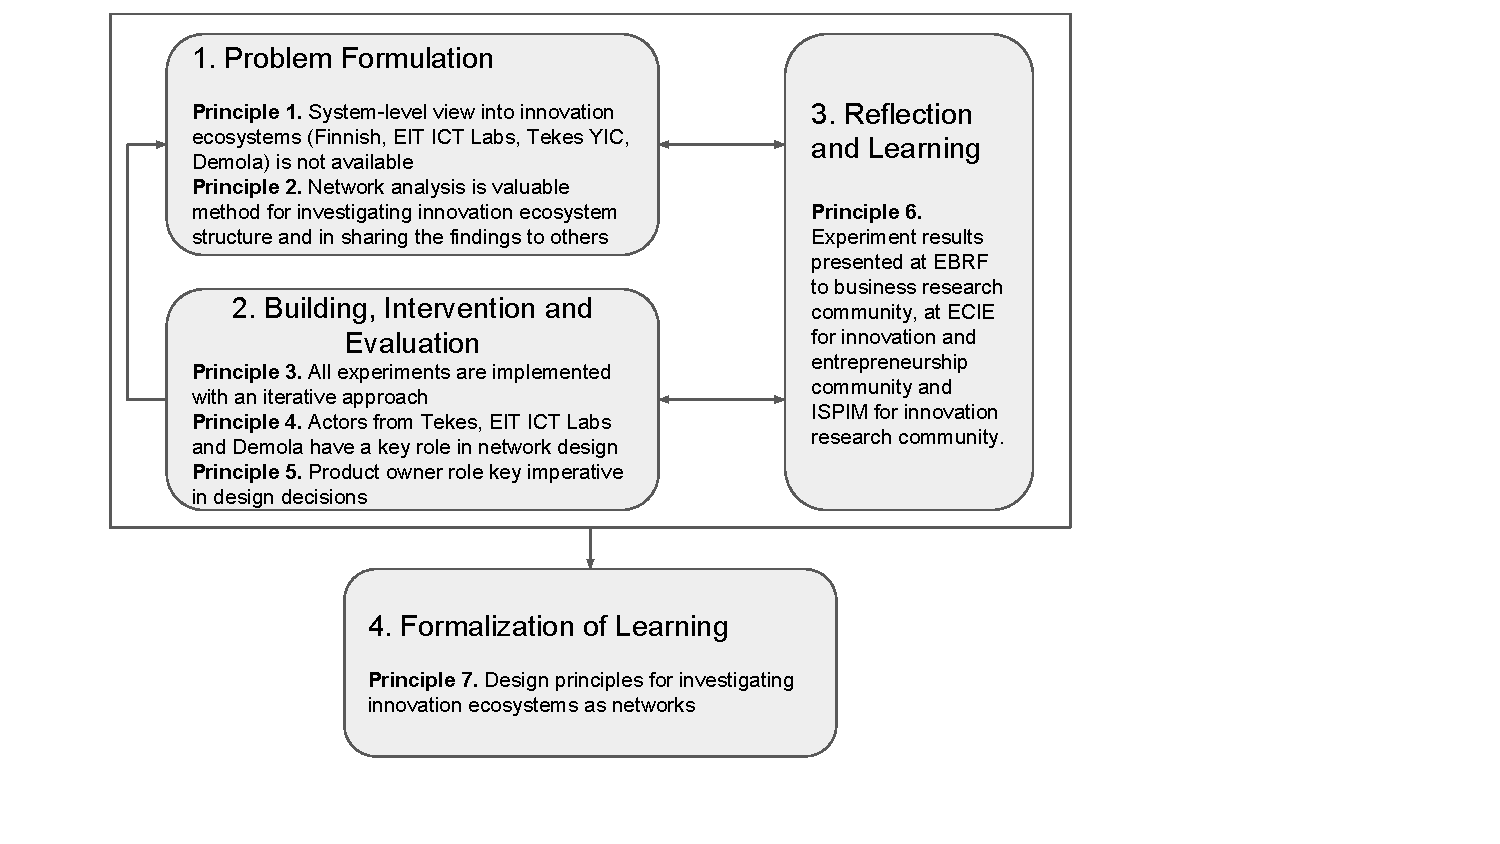
\includegraphics[width=11cm]{diagram/ADR-innovation-ecosystems-as-networks.pdf}
\caption{Action Design Research for investigating innovation ecosystems as networks \citep[following][]{Sein2011ActionResearch}\label{fig:adrapplied}}
\label{fig:ADR-innovation-ecosystems-as-networks}
\end{figure}

\section{Data for network analysis}
\label{sec:networkdata}

The experiments included in this dissertation are based in two main sources of data, the Innovation Ecosystems Network Dataset \citep{Rubens2010LeveragingMoves} and Thomson Reuters SDC. Thomson Reuters SDC is one of the most prominent sources of inter-firm relationships \citep{Schilling2008}. Thomson Reuters SDC is a prime example of a traditional company data sources from which start-ups and growth companies are oftentimes missing. IEN Dataset provides socially curated (or crowd-sourced) rich data about startup and growth companies in almost real-time, though with a public bias. In concert, the two sources of data provide means for creating several complementing views into innovation ecosystems. Following \ref{pub:multiscopicfinland}, the datasets represent different levels of the innovation ecosystem and therefore allow the creation of both microscopic, mesoscopic, macroscopic as well as multiscopic views into the innovation ecosystem \citep{Still2013NetworksFinland}.

More specifically, IEN Dataset includes two subsets of data, Startups and Angels for a microscopic view and Executives and Finance for a mesoscopic view. In addition, Thomson Reuters SDC can be used for data on Deals and Alliances between major enterprises forming the core of the existing business ecosystem, i.e. the macroscopic view. The established enterprises acquire companies and act as sources of talent for startups and growth companies and it is therefore often important to include them in network representations.

Investigation of the Finnish Innovation Ecosystem in \ref{pub:multiscopicfinland} is the first in which we create an aggregate set of data by combining the three different sets on basis of actors that appear in more than one dataset. With the aggregated dataset, we provide an overview into the Finnish Innovation Ecosystem. In our investigations, we use a semi-manual process to aggregate the datasets and call for means to automate the process through string matching \citep{Navarro2001AMatching} to named entity recognition \citep{Finkel2005IncorporatingSampling}.

In \ref{pub:tekesyic}, we further use social media data from Twitter to investigate the structure and interconnections of the Twitter followers of the startups in Tekes Young Innovative Companies program. The list of companies in the program is collected from Tekes website. In \ref{pub:finland}, two complementing sources of data were used: the member list of Finnish Venture Capital Association\footnote{Members of the FVCA, \url{http://www.fvca.fi/en/members}} and ArcticIndex\footnote{ArcticIndex is no longer active. It Was maintained by ArcticStartup, \url{http://arcticstartup.com/}}, a socially constructed dataset of Nordic and Baltic startups.

All of the aforementioned datasets originate from public sources of data. Moreover, proprietary in-house data can be used to represent and analyze innovation ecosystems as networks. Investigation of the Demola platform in \ref{pub:demola} is fully based on in-house data. The first attempt to create a network representation of EIT ICT Labs innovation ecosystem was based on their in-house data as a source. We soon realized, however, that through day-to-day operations, EIT ICT Labs actors know the structure emerging from the in house data by heart. Therefore, we instead decided to use the IEN Dataset to investigate the already existing ecosystem in between the then six co-location cities for insight on the latent social structure as well as  mobility patterns within the co-location cities.

Table~\ref{tab:networkdata} includes a summary of the data sources used in each investigation.

\begingroup
\captionof{table}{Details on collecting and processing data for the experiments}\label{tab:networkdata}
\begin{tabular}{p{3cm} p{2cm} p{4cm} p{3cm}}
\toprule
Experiment & Source & Collecting & Refinement \\
\midrule

Demola &
Project database internal to Demola &
Tailored script for exporting the data from database in use in Drupal CMS &
Unifying project category names \\

Mobile ecosystem &
Innovation Ecosystems Network Dataset (IEND), Thomson Reuters SDC (TR SDC) &
Tailored script that traverses a NoSQL implementation of IEND proxy, TR SDC data imported as an Excel spreadsheet &
Done as part of IEND and Thomson Reuters SDC curation \\

Tekes Young Innovative Companies &
IEND, Twitter &
Tailored scripts for traversing a NoSQL implementation of IEND proxy and accessing Twitter data through a REST API &
Done as part of IEND curation \\

Finnish innovation ecosystem I & 
IEND & 
Tailored script that traverses a NoSQL implementation of IEND proxy &
Done as part of IEND curation \\

Finnish Innovation Ecosystem II  &
IEND, TR SDC &
Tailored script that traverses a NoSQL implementation of IEND proxy, TR SDC data imported as an Excel spreadsheet &
Connecting companies across individual datasets through the creation of unified names \\

EIT ICT Labs &
IEND &
Tailored script that traverses a NoSQL implementation of IEND proxy &
 Done as part of IEND curation \\
\bottomrule
\end{tabular}
\endgroup

\section{Representing innovation ecosystems as networks}
\label{sec:networkrepresentation}

Visual analytics is a key source for requirements in designing the way each of the innovation ecosystems under investigation is represented as a network. Both in the investigations in which we interacted with innovation ecosystem stakeholders as well as in the investigations that the research team conducted independently, we ended up representing the innovation ecosystem under investigation as a multimodal network. Table~\ref{tab:networkdesign} recaps the network modeling decision in the investigations.
  
We do realize, however, that multimodal networks limit the possibilities to apply node and network level metrics to quantify the structural properties of the network as well as the structural roles of the individual actors. At the same time, we observed that using a one-mode network representation of an ecosystem reduces significantly the complexity of the innovation ecosystem under investigation. Moreover, one-mode network representation does not allow for system-level insights of the structural patterns of the innovation ecosystem. The use of one-mode and multimodal networks in concert insists on future development and experimentation. 

\begingroup
\captionof{table}{Network design details for experiments}\label{tab:networkdesign}
\begin{tabular}{p{3cm} p{4cm} p{5cm}}
\toprule
Experiment & Boundary specification & Network modeling \\
\midrule

Demola &
Include the whole project database &
Multimodal network of universities, projects and companies. Connections are formed through project affiliation \\

Mobile ecosystem &
Start from pairs of companies, include their first and second tier connections &
One-mode networks for Thomson Reuters SDC, multimodal networks for IEND \\

Tekes Young Innovative Companies &
Start from companies in Tekes YIC program, include their first and second tier connections &
Multimodal network of companies, key individuals and investors \\

Finnish innovation ecosystem I & 
Start from companies in Finland, include their first tier connections & 
Multimodal network of companies, key individuals and investors \\

Finnish innovation ecosystem II &
Start from companies in Finland, include their first tier connections &
Microscopic, mesoscopic, macroscopic and multiscopic view to Finnish Innovation ecosystem. Macroscopic view is non-directed one mode network, the others are non-directed multimodal networks \\

EIT ICT Labs &
Start from the six EIT ICT Labs co-location centers, include companies having their primary office in one of the cities, include individuals and investors connected to the companies &
Multimodal network of companies, key individuals and investors \\
\bottomrule
\end{tabular}
\endgroup

\section{Analyzing innovation ecosystems as networks}

Network analysis allows for measuring and analyzing the structural properties of innovation ecosystems in all three levels of analysis, system, relationship and actor \citep{Jarvi2016TakingReview}. In system-level, network metrics including density, diameter, and clustering can be applied. Edge weight is a key metric in relationship level and, in addition, detailed relationship properties can be included in network data and used in the analysis of dyads, i.e. pairs of nodes.

Table~\ref{tab:networkanalysis} summarizes the network and node-level metrics we apply in the different experiments. Visual analytics has a focal role in this dissertation and therefore the network metrics have first and foremost served in highlighting actors in significant roles in an innovation ecosystem under investigation. Betweenness centrality is the most used node-level metric. Edge weight is used throughout the investigations. Network metrics allow for comparing the structural properties of individual innovation ecosystems with each other. In this dissertation, network metrics are applied in a number of investigations to describe the structure of innovation ecosystem and, moreover, in the the mobile ecosystem investigation to compare ecosystems with each other.

\begingroup
\captionof{table}{Network design details for experiments}\label{tab:networkanalysis}
\begin{tabular}{p{2.5cm} p{2.5cm} p{3cm} p{3.75cm}}
\toprule
Experiment & Network metrics & Edge metrics & Node metrics \\
\midrule
Demola &
Not applied &
Weight for the number of students representing a university & 
Betweenness for node's "connecting role in the network" \\

Mobile Ecosystem & 
Size, diameter, clustering, density &
Weight for the number of deals and alliances between companies &
Degree, betweenness, clustering coefficient \\

Tekes Young Innovative Companies &
Size &
Dichotomous weight &
Betweenness to "to highlight the individuals, companies and investors that have an important connecting role in the network" \\

Finnish Innovation Ecosystem I & 
Size & 
Dichotomous weight &
Degree, betweenness \\

Finnish Innovation Ecosystem II  &
Size, number of edges, density, diameter &
Dichotomous weight &
Betweenness \\

EIT ICT Labs &
Size, number of edges &
Dichotomous weight &
Degree, betweenness "as a mobility factor to illuminate the potential of individual nodes to serve as bridges between the EIT ICT Labs co-locations" \\
\bottomrule
\end{tabular}
\endgroup

\section{Visualizing innovation ecosystems as networks}

Visual network analysis is an organic part of the approach taken in this dissertation. To reiterate \cite{Freeman2000VisualizingNetworks}, visual network analysis allows for two important tasks in investigating a phenomenon:  first, it supports investigators in observing the social structures emergent in the empirical data representing the phenomenon for insights and, second, it provides a tool for share the findings to others with representations that support co-referencing and the emergence of shared understanding. 

Table~\ref{tab:networkvisualization} recaps the key visualization-related design decisions in the investigations. In all of the investigations, we have used a force-driven algorithm to lay out the nodes. More specifically, we have applied the two variants of Force Atlas algorithm implemented in Gephi \citep{Bastian2009Gephi:Networks}. A consistent color scheme for nodes was established already in the first investigation. The investigative team observed that using colors to identify node types--green for investors, red for companies and blue for individuals--over time eases the visual investigation of networks as observers become familiar with the semantics of the colors. We further note that consistency of the network layout is also an important analysis process design objective when visual network analytics is used to analyze an innovation ecosystem over time. We will come back to this topic in relation to the Ostinato Model in Chapter~\ref{ch:ostinato}.

\begingroup
\captionof{table}{visualization details for the experiments}\label{tab:networkvisualization}
\begin{tabular}{p{3cm} p{3cm} p{6cm}}
\toprule
Experiment & Layout & Visual properties \\
\midrule
Finnish Innovation Ecosystem I & 
Force-driven & 
Node color represents its type: red for companies, green for investors and blue for individuals  \\
Mobile Ecosystem &
Force-driven &
Node color represents its type: red for companies, green for investors and blue for individuals  \\
Tekes Young Innovative Companies &
Force-driven &
Node color represents its type: red for companies, green for investors and blue for individuals  \\
Finnish Innovation Ecosystem II  &
Force-driven &
Node color represents its type: gold for Finnish companies, red for foreign companies, green for investors and blue for individuals  \\
Demola &
Force-driven, dynamic when animating network evolution &
For projects, node color represents its membership in network cluster; company nodes are represented in light green \\
EIT ICT Labs &
Force-driven &
Node color represents its type: red for companies, green for investors and blue for individuals  \\
\bottomrule
\end{tabular}
\endgroup

\section{Design guidelines for network representation and analysis}
\label{sec:designguidelines}

Through the experiments reviewed in Chapter~\ref{ch:experiments}, we have investigated a number of innovation ecosystems as networks. Next, to generalize the observations we have made through the experiments and to support future efforts to model and represent innovation ecosystems as networks, we provide a set of design guidelines stemming from the experiments to guide analysts and researchers taking a data-driven visual network analytics approach to innovation ecosystem investigations.

\subsection{Modeling innovation ecosystems as networks}
The decisions done in network modeling depicts the options for using different node-level metrics in analysis. Directed one-mode network with weighted connections allows the use of the widest range of metrics. In all of the investigations included in this dissertation, however, together with several ensembles of investigators, we have decided to represent innovation ecosystems with multimodal networks.

\guideline{1a}{Companies, key individuals, and investors are the basic entities in innovation ecosystem network representations}

\guideline{1b}{Multimodal networks provide an intuitive starting point for representing innovation ecosystem as network for a holistic overview of its structure}

\guideline{1c}{One-mode networks allow for detailed quantitative and statistical analysis with the expense of reducing the complexity of the ecosystem}

\guideline{1d} {Edge direction and weight introduce additional means to utilize network metrics to support the analysis}

\subsection{Analyzing the networks}

In visual analytics, network metrics are used to highlight actors in different structural positions in the network. Node degree, indegree and outdegree are the most simple metrics. Betweenness centrality is a useful metric also in the context of multimodal networks. \cite{Hansen2011AnalyzingWorld} refer to betweenness centrality with as ``Bridge Scores for Boundary Spanners''. Moreover, additional network metrics become available when an innovation ecosystem is represented as a directed one-mode network. 

\guideline{2a}{Node degree identifies actors with the largest amount of connections.}

\guideline {2b}{Outdegree identifies the most active actors.}

\guideline {2c}{Indegree is the simplest metric for prestige or authority.}

\guideline{2d}{Betweenness highlights nodes that have a bridging role in the network.}

\subsection{Visualizing the networks}

We have applied force-driven layout in all of the investigations included in this dissertation. A key reason for this is that the author of this dissertation together with a the core team has remained the same throughout the investigation and have proposed the use of force-driven layout. Nevertheless, all the other stakeholders in the investigations have also found the basic principle behind the force-driven layout to be intuitive. To our experience, the force-driven layout allows for the visual identification of network clusters and actors bridging the clusters.

Visual consistency is important in investigations where different network representation of the innovation ecosystem under investigation are created. We have established a consistent color scheme for innovation ecosystem actors. Even more important is to maintain the positions of the individual actors and clusters of actors in between different representations, snapshots and rounds of investigations. We discuss this in more detail when describing the Ostinato Model in Chapter~\ref{ch:ostinato}.

Filtering is a key approach to reduce complexity in visual representations of innovation ecosystem networks. At best, an  investigator analyzing an innovation ecosystem as network is able to filter the network throughout the sensemaking process. More on this in section on interactive exploration. To allow expressive filtering, supporting data should be included into nodes and edges when creating the network.  

\guideline{3a}{Force-driven network layout allows insight on the overall structure, key patterns as well as the roles of individual actors of the network.}

\guideline{3b}{Establish a consistent and intuitive color scheme to differentiate node type. We use red for companies; green for finance organizations; and blue for key individuals (founders, C-level employees, board members).}

\guideline{3c}{Keep network layout constant within and in between individual investigations to ease the investigators to establish a mental model of the innovation ecosystem network representation.}

\guideline{3d}{Apply filtering to reveal the patterns related to the phenomenon under investigation.}

\subsection{Investigating network evolution}

Two key approaches exist for investigating the development of network structure, often referred to as network evolution \citep[cf.][]{Ahuja2012TheNetworks}. First, the development of network metrics can be represented on a timeline. In \ref{pub:mobileecosystem}, we use small multiple timelines, an application of small multiples \citep{Heer2012InteractiveAnalysis,Tufte1983VisualInformation}, to represent the development of a number of networks to support their comparison and in supporting gaining insight on network evolution. In \ref{pub:demola}, we developed animation of the evolution of Demola's innovation ecosystem as a network. We see that supporting the investigations of network evolution through visual analytics provides a major venue for future research and development.

\guideline{4a}{Small multiple timelines provide insights on change in network and actor level metrics.}

\guideline{4b}{Network animation allows additional insights on the evolution of an innovation ecosystem.}

\subsection{Interactive exploration}

To reiterate, visual network analytics is a process \citep{Heer2012InteractiveAnalysis,Keim2010MasteringAnalytics}. Therefore, supporting the processual nature of an investigation is imperative in selecting tools for the analytics process. Gephi is the main tool in use in all of the investigations in this dissertation. In addition to network-specific tools, network and node metrics can be explored with interactive tools from spreadsheet processors to business intelligence tools including Tableau and others. It is imperative to extend the ability to interact to upstream analysis, i.e. data transformations, boundary specification and eventually data-collection routines. The ability to interact with the different phases of the data-driven visual network analytics process at the core of the Ostinato Model.

\guideline{5a}{Support both top-down and bottom up analysis: Start with what you know, then grow \citep{Heer2005Vizster:Networks}. Overview first, details on demand \citep{Shneiderman1996TheVisualizations}.} 

\guideline{5b}{Allow for experimenting with the different node metrics in defining visual properties for nodes.}

\guideline{5c}{Enable filtering nodes and edges on basis of parameters relevant to the investigation. Importantly, this calls for including node and edge properties that support filtering.}

\guideline{5d}{Seek means to allow for interacting with boundary specification.}

\subsection{Sharing the findings}

Interactivity is priority also when selecting the tools for provisioning the visualizations to investigators and others interested in the findings. We have used e.g. GEXF.js\footnote{JavaScript GEXF Viewer for Gephi, \url{https://github.com/raphv/gexf-js}}, an interactive exploration tool running on  a Web browser, for provisioning network visualization.

\guideline{6}{Provision the outputs of the data-driven visual network analytics process with high-interaction visualization tools that support sensemaking and storytelling.}
